\documentclass[tikz,border=12pt]{standalone}
% Shared visual language for standalone EMT block diagrams.
\usepackage{amsmath}
\usetikzlibrary{arrows.meta,backgrounds,calc,fit,positioning}

\tikzset{
    emt diagram/.style = {>={Stealth[length=2.4mm]}},
    line/.style        = {semithick, rounded corners=6pt},
    block/.style       = {draw, semithick, fill=white,
                          minimum height=1cm, minimum width=2.3cm},
    hblock/.style      = {block, minimum width=2.24cm, minimum height=1.3cm},
    vblock/.style      = {block, minimum width=1.3cm, minimum height=2.24cm},
    sum/.style         = {draw, semithick, fill=white, circle,
                          inner sep=2.6pt},
    signal/.style      = {circle, fill, inner sep=1.4pt,
                          label distance=3pt},
    sig/.style         = {font=\small},
    pm/.style          = {font=\scriptsize},
    wire jump/.style   = {line,
                          preaction={draw=white, line width=3pt,
                                     line cap=round}},
    enclosure/.style   = {draw, dashed, semithick, rounded corners=4pt},
    operator enclosure/.style = {enclosure, inner xsep=7mm, inner ysep=6mm}
}


\begin{document}
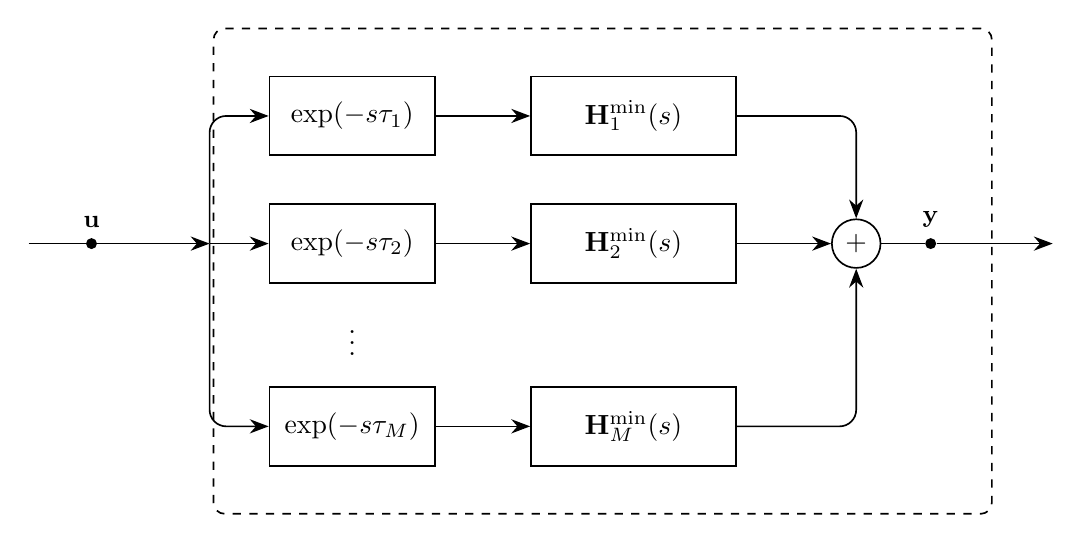
\begin{tikzpicture}[emt diagram]

% One branch per mode: own delay into the fitted mode matrix, summed.
\node[block, minimum width=2.1cm] (D2) {$\exp(-s\tau_2)$};
\node[block, minimum width=2.1cm, above=0.6cm of D2] (D1) {$\exp(-s\tau_1)$};
\node[block, minimum width=2.1cm, below=1.3cm of D2] (DM) {$\exp(-s\tau_M)$};
\node at ($(D2)!0.5!(DM)$) {$\vdots$};

\node[block, minimum width=2.6cm, right=1.2cm of D1]
    (H1) {$\mathbf{H}^{\min}_1(s)$};
\node[block, minimum width=2.6cm, right=1.2cm of D2]
    (H2) {$\mathbf{H}^{\min}_2(s)$};
\node[block, minimum width=2.6cm, right=1.2cm of DM]
    (HM) {$\mathbf{H}^{\min}_M(s)$};
\foreach \m in {1, 2, M}
    \draw[->, line] (D\m.east) -- (H\m.west);

% Fan-out from a single internal point
\coordinate (split) at ($(D2.west)+(-0.75, 0)$);
\draw[->, line] (split) -- (D2.west);
\foreach \b in {D1, DM}
    \draw[->, line] (split) |- (\b.west);

% Fan-in to the modal sum
\node[sum, right=1.2cm of H2] (add) {$+$};
\draw[->, line] (H2.east) -- (add.west);
\draw[->, line] (H1.east) -| (add.north);
\draw[->, line] (HM.east) -| (add.south);

% Output node (owned by this model) with port arrow out
\node[signal, label={[sig]above:$\mathbf{y}$}, right=0.55cm of add] (yout) {};
\draw[line] (add.east) -- (yout);
\draw[->, line] (yout) -- ++(1.55, 0);

% Input node (owned externally) with port arrow into this model
\node[signal, label={[sig]above:$\mathbf{u}$}] (uin)
    at ($(split)+(-1.5, 0)$) {};
\draw[->, line] ($(uin)+(-0.8, 0)$) -- (split);

% Model enclosure: fixed padding around model-owned blocks and output variable
\begin{scope}[on background layer]
    \node[operator enclosure, fit=(D1)(D2)(DM)(H1)(H2)(HM)(add)(yout)] {};
\end{scope}

\end{tikzpicture}
\end{document}
